\documentclass{beamer}

\usepackage[export]{adjustbox}
\usepackage{amsmath,amsthm,amssymb,amsfonts}
\usepackage[backend=biber, style=apa]{biblatex}
\usepackage{caption}
\usepackage[T1]{fontenc}
\usepackage{graphicx}
\usepackage{lmodern}
\usepackage[outputdir=dist]{minted}
\usepackage{ru}
\usepackage{url}
\usepackage{xpatch,letltxmacro}
\usepackage{stmaryrd}
\usepackage{wrapfig}

\newcommand{\cd}[1]{\texttt{#1}}

\setminted{fontsize=\small}
\LetLtxMacro{\cminted}{\minted}
\let\endcminted\endminted
\xpretocmd{\cminted}{\RecustomVerbatimEnvironment{Verbatim}{BVerbatim}{}}{}{}

\mode<presentation>{}

\title{\textbf{Compiler Construction: Lexical analyses}}

\author{Quinten Cabo, Marijn van Wezel}

\institute{Radboud University Nijmegen}
\date{27 February 2024}

\begin{document}

\setbeamercovered{transparent}
\setbeamercolor{alerted text}{fg=black}
\setbeamerfont{alerted text}{series=\bfseries}

\frame{\titlepage}

\begin{frame}
  \frametitle{What was a compiler again?}
  
  \begin{center}
  \only<1>{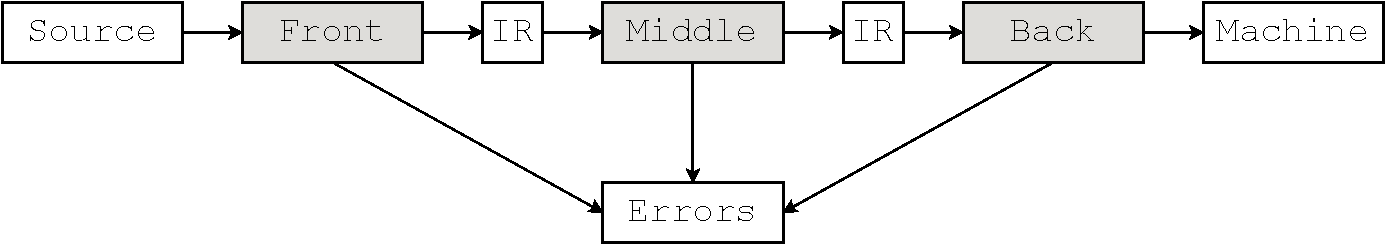
\includegraphics[width=300px]{figures/compiler_phases.pdf}}
  \only<2>{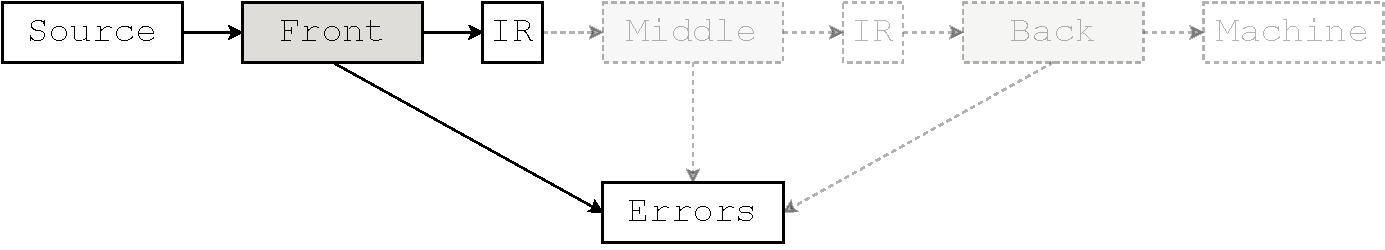
\includegraphics[width=300px]{figures/compiler_phases_highlighted.pdf}}
  \end{center}
\end{frame}

\begin{frame}<1>[label=the-goal]
  \frametitle{The goal}

  \begin{itemize}[<+->]
    \item \alert<1>{Given some arbitrary string of characters,}
    \item \alert<2>{analyse this string,}
    \item \alert<3>{produce an abstract syntax tree,}
    \item \alert<4>{or give an error.}
  \end{itemize}
\end{frame}

\begin{frame}[fragile]
  \frametitle{String of characters: Examples}

  \begin{onlyenv}<1>
    \begin{minted}{text}
      sum(l:[Int]): Int {
        if (isEmpty(l.tl)) {
          return l.hd;
        }

        return l.hd + sum(l.tl);
      }
    \end{minted}
  \end{onlyenv}

  \begin{onlyenv}<2>
    \begin{minted}{text}
      product(list:[Int]): Int {
        if (isEmpty(list)) {
          return 1;
        }

        return list.hd * product(list.tl);
      }
    \end{minted}
  \end{onlyenv}

  \begin{onlyenv}<3>
    \begin{minted}{text}
      product(list:[Int]: Int {
        if (isEmpty(list)) {
          return 1;
        }

        return list.hd * product(list.tl);
      }
    \end{minted}
  \end{onlyenv}
\end{frame}

\againframe<2>{the-goal}

\begin{frame}
  \frametitle{Analysis: Haskell}

  We chose \textit{Haskell} to implement our parser (and the rest of our compiler):

  \begin{itemize}[<+->]
    \item Algebraic data types;
    \item High level of abstraction;
    \item Good tooling and library support;
    \item \textbf{Functional parser combinators}.
  \end{itemize}
\end{frame}

\begin{frame}
  \frametitle{Analysis: Functional parser combinators}

  Parser combinators work through \textit{function composition}.

  \begin{center}
    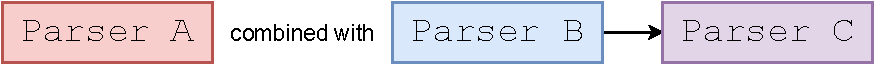
\includegraphics[width=300px]{figures/parser_combinator.pdf}
  \end{center}
\end{frame}

\begin{frame}
  \frametitle{Analysis: megaparsec}

  \begin{figure}
    \begin{center}
      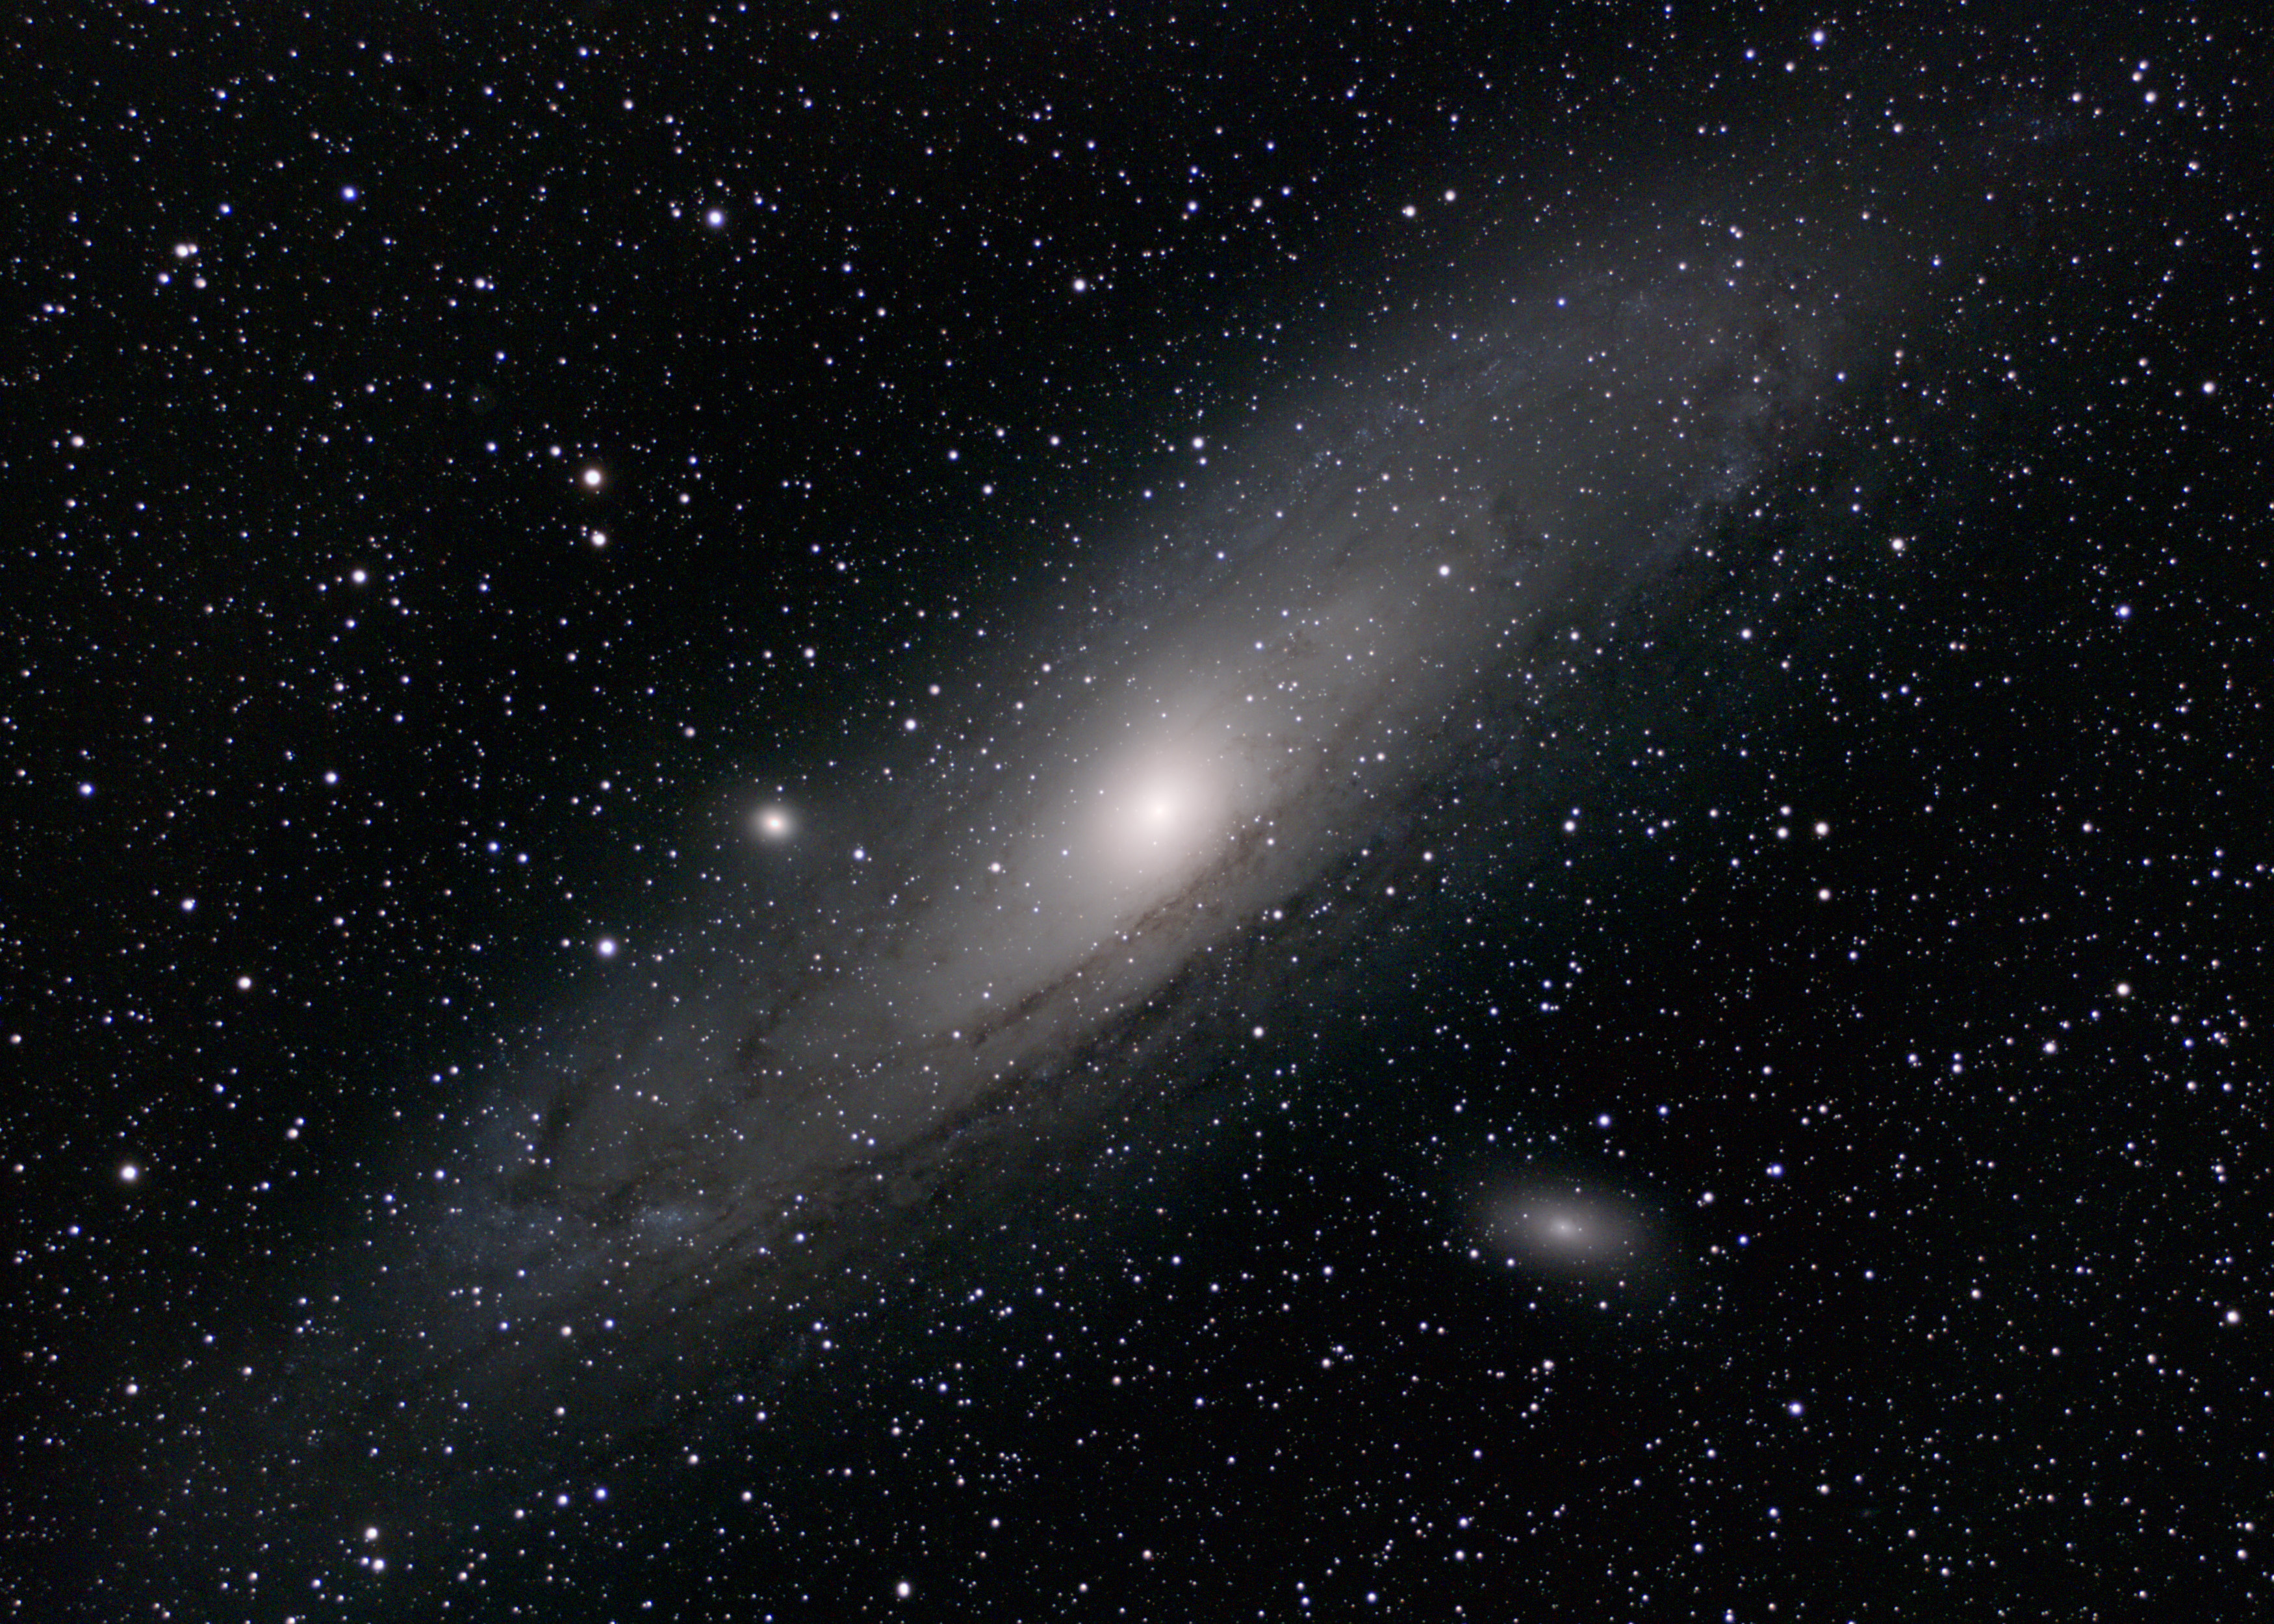
\includegraphics[width=0.7\textwidth]{figures/andromeda.jpg}
      \captionsetup{labelformat=empty}
      \caption{The Andromeda Galaxy is roughly one \textbf{megaparsec} away (Torben Hansen, CC-BY-2.0).}
    \end{center}
  \end{figure}
\end{frame}

\begin{frame}
  \frametitle{Analysis: megaparsec}

  \begin{itemize}[<+->]
    \item Informal successor of Parsec;
    \item Does much of the heavy lifting;
    \item Large collection of combinators;
    \item Decent error messages out-of-the-box;
    \item \mintinline{text}{makeExprParser} 
  \end{itemize}
\end{frame}

\begin{frame}
  \frametitle{Analysis: Tokenless parsing}

  We decided to use a tokenless (lexer-less) parsing approach.

  \begin{itemize}[<+->]
    \item Works well with parser combinators
    \item Good support by megaparsec
  \end{itemize}
  % whitespace
  % symbols
  % examples
  % megaparsec only removes whitespace at end
\end{frame}

\begin{frame}[fragile]
  \frametitle{Analysis: Tokenless parsing}

  Tokens are parsed using special \mintinline{text}{symbol} parsers.

  \begin{center}
    \begin{minted}{haskell}
      -- ...

      tTrue :: Parser T.Text
      tTrue = symbol "true"

      tFalse :: Parser T.Text
      tFalse = symbol "false"

      tEmptyList :: Parser T.Text
      tEmptyList = symbol "[]"

      -- ...
    \end{minted}
  \end{center}
\end{frame}

\begin{frame}[fragile]
  \frametitle{Analysis: Tokenless parsing}

  Token parsers strip whitespace (spaces, tabs, comments) at the end of the input:

  \begin{center}
    \begin{minted}{haskell}
      whitespace = L.space
        space1
        (L.skipLineComment "//")
        (L.skipBlockComment "/*" "*/")

      tColon :: Parser T.Text
      tColon = symbol ":"

      -- tColon parses ":", but also ": /* Parsers are fun */"
    \end{minted}
  \end{center}
\end{frame}

\begin{frame}[fragile]
  \frametitle{Analysis: Tokenless parsing}

  \begin{center}
    \begin{minted}{haskell}
      pProgram :: Parser Program
      pProgram = L.whitespace *> some pDecl
    \end{minted}
  \end{center}
\end{frame}

\begin{frame}[fragile]
  \frametitle{Analysis: Generating expression parsers}

  \begin{center}
    \begin{minted}{haskell}
      operatorTable :: [[Operator Parser Expr]]
      operatorTable =
        [ [ Postfix (UnaryOp (FieldAccess HeadField) <$ try (L.tDot <* L.tHead))
          , Postfix (UnaryOp (FieldAccess TailField) <$ try (L.tDot <* L.tTail))
          ]
        , ...
        ]

      pTerm :: Parser Expr
      pTerm = choice
        [ try $ L.parens pExpr
        , try pFunctionCall
        , try pAssignExpr
        , try pLiteralExpr
        , try pVariableExpr
        ]

      pExpr :: Parser Expr
      pExpr = makeExprParser pTerm operatorTable
    \end{minted}
  \end{center}
\end{frame}

\begin{frame}[fragile]
  \frametitle{Analysis: Testing the parser}

  \begin{center}
    \begin{minted}[fontsize=\footnotesize]{haskell}
      exprSpec :: Spec
      exprSpec = do
        describe "Parser.Expr" $ do
          describe "pExpr" $ do
            it "parses a term" $ do
              parse pExpr "test.spl" "1" 
                `shouldParse` LiteralExpr (IntLit 1)
              parse pExpr "test.spl" "a = 'b'" 
                `shouldParse` AssignExpr (Identifier "a" Nothing) (LiteralExpr $ CharLit 'b')
              parse pExpr "test.spl" "ident"
                `shouldParse` VariableExpr (Identifier "ident" Nothing)
              parse pExpr "test.spl" "(a + b)"
                `shouldParse` BinOp Add 
                    (VariableExpr (Identifier "a" Nothing))
                    (VariableExpr (Identifier "b" Nothing))
    \end{minted}
  \end{center}

  
\end{frame}

\begin{frame}[fragile]
  \frametitle{Analysis: Testing the parser}

  \begin{center}
    \begin{minted}[fontsize=\footnotesize]{text}
      Parser.Expr
        pExpr
          parses a term [v]
          parses a simple unary expression [v]
          parses a simple binary expression [v]
          parses an expression [v]
    \end{minted}
  \end{center}
\end{frame}

\againframe<3>{the-goal}

\begin{frame}
  \frametitle{Abstract syntax tree: design goals}

  \begin{itemize}[<+->]
    \item We started with the design of our AST, and based our parser on that;
    \item Tried to make the AST only be able to represent syntactically valid programs;
    \item Tried to make the AST as simple as possible;
    \item \mintinline{haskell}{data} type is Haskell.
  \end{itemize}
\end{frame}

\begin{frame}[fragile]
  \frametitle{Abstract syntax tree: example}

  \begin{minted}{haskell}
    data Stmt =
      ReturnStmt (Maybe Expr)           -- return a;
    | IfStmt Expr [Stmt] (Maybe [Stmt]) -- if (a) {b} else {c}
    | WhileStmt Expr [Stmt]             -- while (a) {b}
    | ExprStmt Expr                     -- a;
    | VarStmt (Maybe Type) String Expr  -- var hello = 'w':'o':'r':'l':'d':[]
    deriving (Eq, Show)
  \end{minted}
\end{frame}

\againframe<4>{the-goal}

\begin{frame}[fragile]
  \frametitle{Error reporting}

  Megaparsec generates decent error messages out of the box:

  \begin{minted}{text}
    examples/product_parse_error.spl:1:19:
      |
    1 | product(list:[Int]: Int {
      |                   ^
    unexpected ':'
    expecting ')' or ','
  \end{minted}

  But also has support for custom error messages, and even error recovery. We have not yet implemented this.
\end{frame}

\begin{frame}[fragile]
  \frametitle{Pretty printer}

  \begin{onlyenv}<1,2>
  \begin{minted}{text}
    fib(n : Int) : Int {
      if (n == 0) {return 0;}


if    (n == 1) {
   if           (true)           {print('h':'i':[]);}
return 1;}return (fib(n - 1) + fib(n - 2));  }
    \end{minted}
  \end{onlyenv}

\begin{onlyenv}<3>
  \begin{minted}{text}
  fib(n : Int) : Int {
    if (n == 0) {
        return 0;
    }
    if (n == 1) {
        if (true) {
            print('h':'i':[]);
        }
        return 1;
    }
    return fib(n - 1) + fib(n - 2);

  }
    \end{minted}
  \end{onlyenv}
  \only<2>{
\includegraphics[width=55px]{figures/barf.png}}
  \only<3>{
\includegraphics[width=55px]{figures/happy.png}}
\end{frame}

\begin{frame}[fragile]
  % comments are hard
  \frametitle{Pretty printer - Comments}
    \begin{onlyenv}<1>
  \begin{minted}{text}
    fib(n : Int) : Int {
      if (n == 0) {return 0;}
    
/*    /| ________________
O|===|* >________________>
      \|                         */

if    (n == 1) { //                                  h   i 
   if /* always true? */  (true) /* hi */    {print('h':'i':[]);}
return 1;}return (fib(n - 1) + fib(n - 2));  }
    \end{minted}
  \end{onlyenv}
\begin{onlyenv}<2>
  \begin{minted}{text}
  fib(n : Int) : Int {
    if (n == 0) {
        return 0;
    }
    if (n == 1) {
        if (true) {
            print('h':'i':[]);
        }
        return 1;
    }
    return fib(n - 1) + fib(n - 2);

  }
    \end{minted}
  \end{onlyenv}
  \only<2>{
\includegraphics[width=55px]{figures/kinda_sad.png}}

  \begin{onlyenv}<3>
  \begin{minted}{text}
    type Program = ([Decl], [Comment])
                        -- start  end 
    data Comment = Single Int Int Int Int String
                 | Multi  Int Int Int Int String
    % Make the symbol parser fix it
  \end{minted}
  \end{onlyenv}

\end{frame}


\begin{frame}
  \begin{center}Questions?\end{center}
\end{frame}

\end{document}

